%-*-coding: utf-8-*-
\chapter{Решение задачи поиска расстояний между каждой парой вершин графа}

В этой главе будет приведено решение задачи поиска расстояний между каждой парой вершин. В начале главы будет краткий обзор предметной области, далее будут приведены два решения для поиска пути, а после будет приведено решение задачи для социальных неориентированных невзвешенных графов, которое будет сочетать в себе несколько подходов и идей, изложенных в предыдущих алгоритмах. 

\FloatBarrier
\section{Обзор существующих решений}

\subsection{Алгоритм Флойда}
Одним из наиболее известных алгоритмов, который применяется для решения данной задачи является алгоритм Флойда. Этот алгоритм использует идею динамического программирования и выполняется за $O(V^3)$. Основная идея состоит в обновлений пути между двумя текущими вершинами выбором некоторой вершины, через которую может пройти потенциальный кратчайший путь. Псевдокод алгоритма приведен ниже. 

\FloatBarrier
\begin{algorithm}
\caption{Алгоритм Флойда}\label{floyd}
\begin{algorithmic}[1]
\Procedure{Floyd}{$G$}
\State $dist\gets \left\{ {   \left\{ {\infty \ldots \infty}\right\}  \ldots \left\{ {\infty \ldots \infty}\right\} }\right\}$
\For{$e \in G.edges $}
	\State $dist[e.from][e.to] \gets e.w$
\EndFor 
\State
\For{$i = 0$ to $|G.vertices| $}
	\For{$u = 0$ to $|G.vertices| $}
		\For{$v = 0$ to $|G.vertices| $}
			\State $dist[u][v] \gets \min(dist[u][v], dist[u][i] + dist[i][v])$
		\EndFor
	\EndFor
\EndFor
\State \textbf{return} $dist$
\EndProcedure
\end{algorithmic}
\end{algorithm}

\FloatBarrier
\subsection{Альтернативы}
В некоторых случаях оказываются эффективны другие подходы. Например, можно для каждой вершины по отдельности запустить некоторый алгоритм поиска кратчайшего пути до всех остальных вершин. Для случая неотрицательных ребер можно применить алгоритм Дейкстры, в более общем случае может быть применен Беллман-Форд. Кроме вышеприведенных подходов также известен алгоритм Джонсона, который работает на графах без циклов отрицательного веса и находит кратчайшие расстояния за время $O(V^2 \log(V) + VE)$. Все эти алгоритмы оказываются эффективны в случае разреженных графов.

В последующих подходах в качестве основы для параллельного алгоритма будет использоваться именно идея подсчета расстояний либо для каждой вершины по отдельности, либо подсчета расстояний для групп вершин одновременно. И все нижеперечисленные алгоритмы, как и описанные выше альтернативы, хорошо работают на разреженных графах.

\FloatBarrier
\section{Наивная параллельная версия}
Первая версия заключается исключительно в запуске Беллмана-Форда для каждой из вершин. При этом заметим, что так как каждый из них независим друг от друга, то можем эти запуски распараллелить между собой. В качестве простого критерия остановки разделения множества для обработки будем использовать некоторую константу $threshold$. Кроме того, важно отметить, что необходимо выбирать наиболее подходящую реализацию параллельного Беллмана-Форда в зависимости от типа графа. К примеру, в случае разреженного графа с положительными ребрами нам подойдет последняя реализация, основанная на параллельном обхода в ширину. Таким образом, псевдокод из себя представляет следующее.


\FloatBarrier
\begin{algorithm}
\caption{Наивная параллельная версия}\label{all_pairs_par1}
\begin{algorithmic}[1]
\Procedure{AllPairsPar1}{$G$}
\State \textbf{return} {\Call {HandleVertices}{$G, 0, |G.vertices|$}}
\EndProcedure
\State
\Procedure{HandleVertices}{$G, startVertex, endVertex$}

\If {$endVertex - startVertex < threshold$} 
	\State $distances \gets$ Запустить параллельную версию Беллмана-Форда для каждой вершины из полуинтервала $[startVertex, endVertex)$ 
	\State \textbf{return} $distances$	
\Else	
	\State $midVertex \gets (startVertex + endVertex) / 2$ 
	\State \begin{varwidth}[t]{\linewidth}fork2(\par
        \hskip\algorithmicindent {\Call {HandleVertices}{$G, startVertex, midVertex$}},\par
        \hskip\algorithmicindent {\Call {HandleVertices}{$G, midVertex, endVertex$}});
      \end{varwidth}
	
\EndIf

\EndProcedure

\end{algorithmic}
\end{algorithm}

\FloatBarrier
\section{Параллельный алгоритм для объединенного графа}
Развитием предыдущей идеи является наблюдение, что для некоторого набора вершин можем построить общий граф и запустить на нем Беллмана-Форда, что потенциально может повысить производительность за счет высокой параллельности для общего графа, в то время как для каждого отдельно взятого Беллмана-Форда она низкая. Кроме того, это избавит нас от выбора константы для предыдущей версии, что упростит использование алгоритма для пользователя. 

Идея заключается в запуске алгоритма Беллман-Форд на графе, вершины которого описываются двумя значениями - текущей вершины в обходе и вершины, из которой этот обход начался (иными словами, вершины, из которой мы ищем кратчайшие расстояния). После построения графа будет достаточно запустить обход, при этом положив в Frontier все вершины вида $(i, i)$. В итоге кратчайшее расстояние для вершины $(i, j)$ будет интерпретироваться как кратчайшее расстояние от вершины $i$ до вершины $j$ в исходном графе. Описанный алгоритм иллюстрирован на примере простейшего графа из 3 вершин на рисунке \ref{floyd_par_common_graph}. 
\FloatBarrier

\begin{figure}[h]
\caption{Пример преобразования для простейшего графа}
\label {floyd_par_common_graph}
\centering
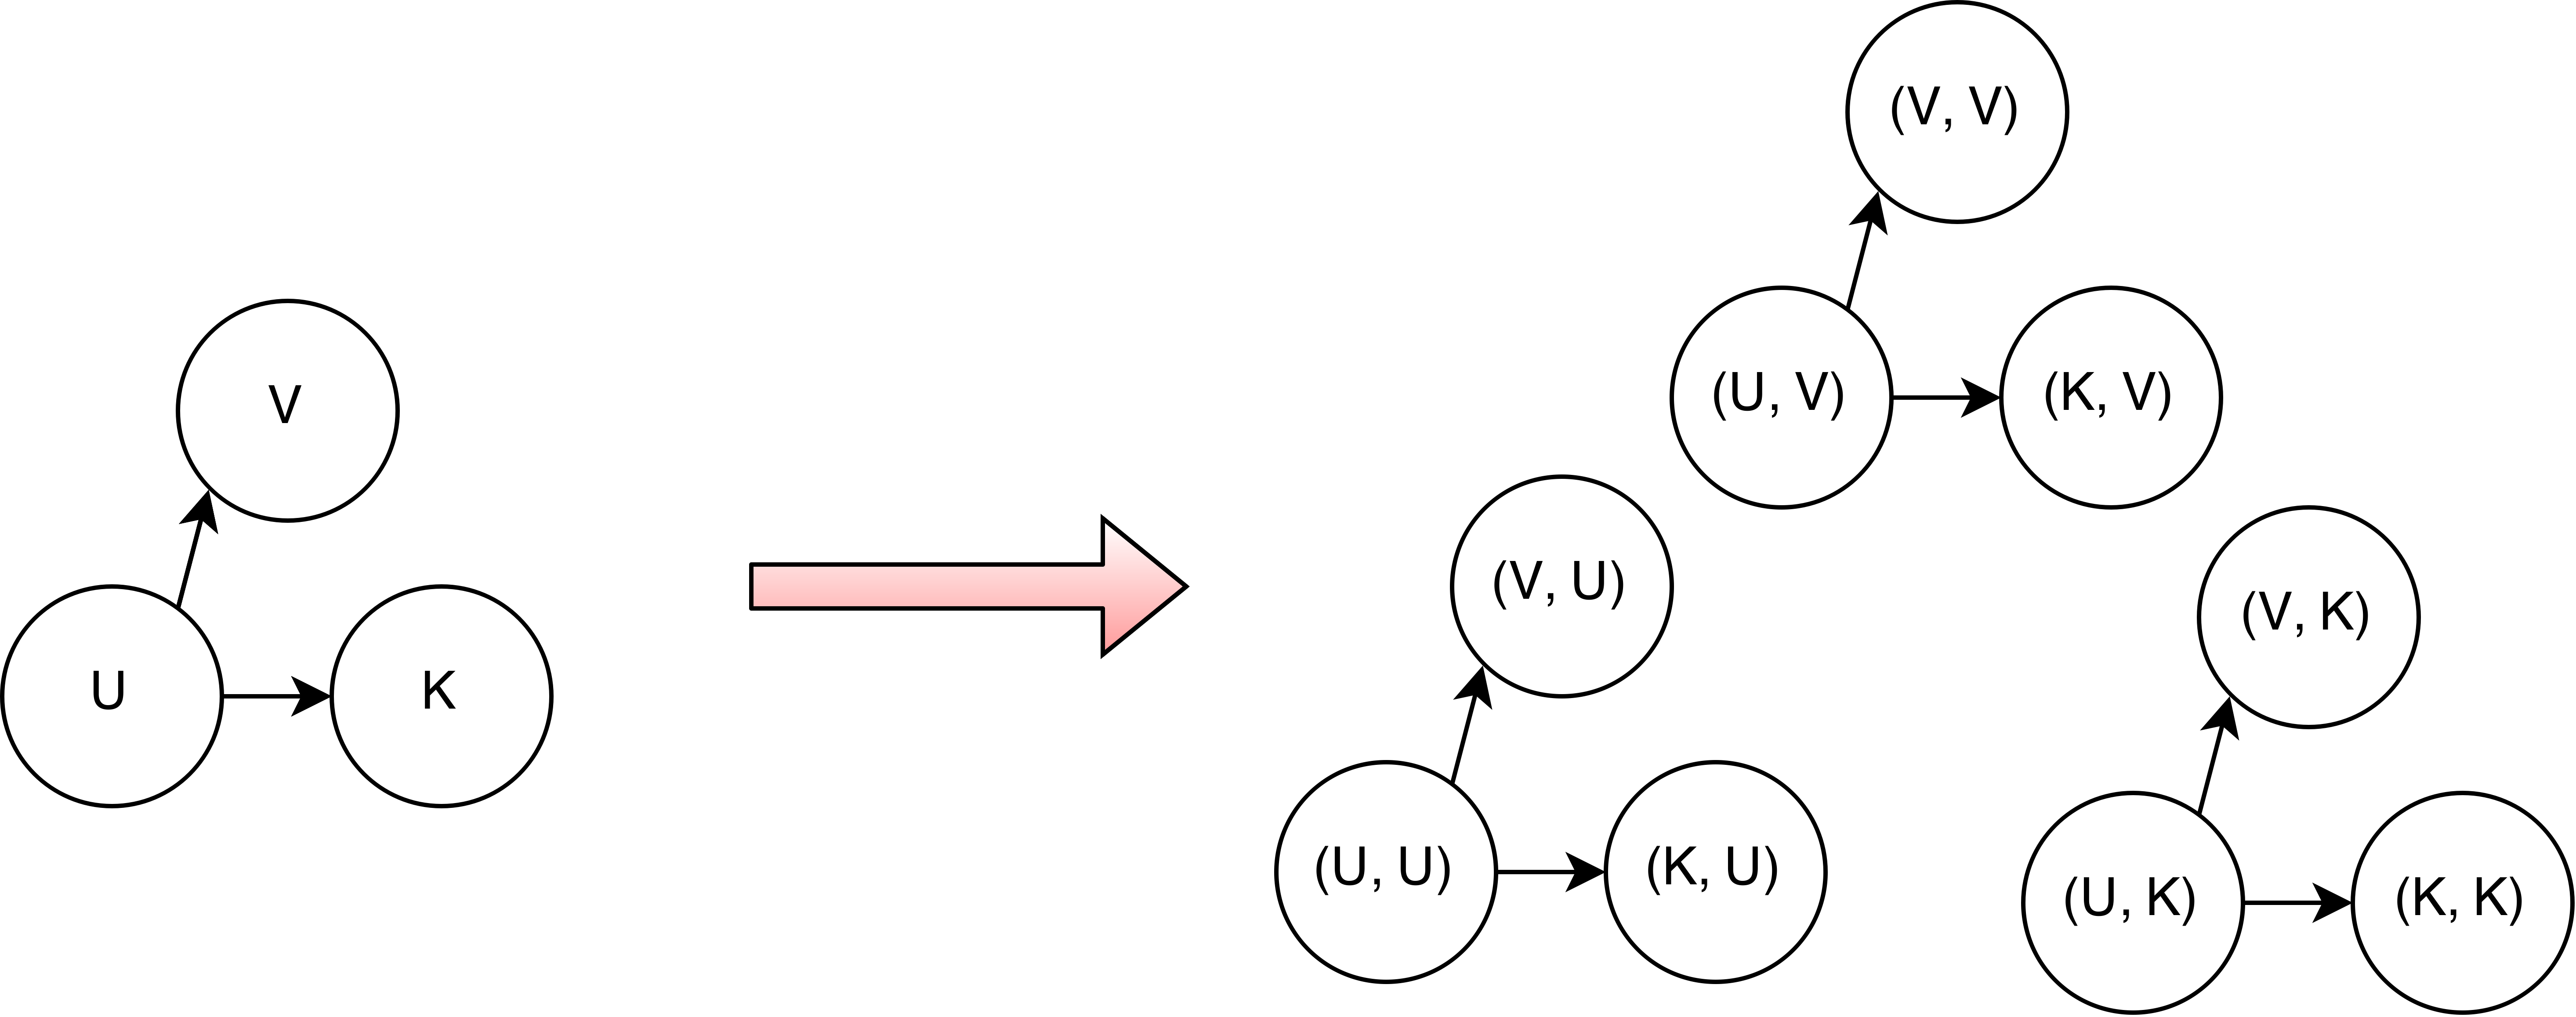
\includegraphics[width=0.9\textwidth]{img/floyd_par_2.png}
\end{figure}
\FloatBarrier

Однако, как будет показано позднее, такой подход на практике оказался немного медленнее наивной версий. Но при этом идея обработки ряда вершин одновременно легла в основе следующего алгоритма для социальных графов. 
\FloatBarrier
\section{Параллельный алгоритм для социальных графов}
В данной главе будет рассмотрен алгоритм поиска кратчайшего пути между каждой парой вершин для графов реальных социальных сетей. При этом рассмотренный граф будет невзвешенный и неориентированный. Кроме того, в этой главе будет рассмотрена производительность алгоритма на примере реальных подграфов известных социальных сетей, таких как Twitter и Slashdot\cite{STANFORDGRAPHS}.

\FloatBarrier
\subsection{Идея алгоритма}
В графах для социальных сетей известна одна эвристика, которая называется "Теория шести рукопожатий". В ее основе лежит тот факт, что практически любые два человека на земле знакомы не более, чем через пятерых промежуточных людей. Таким образом, выбрав некоторую случайную вершину, мы сможем добраться от нее до большинства других вершин не более, чем за 6 ребер. Воспользуемся этой эвристикой в нашем алгоритме и выберем вершину наибольшей степени в качестве базовой. И рассмотрим два множества - вершины, которые находятся на расстоянии не более 6 от базовой ("большое" множество) и все остальные вершины ("меньшее" множество). Кроме того, будем обрабатывать эти два множества различным образом - для меньшего будем запускать параллельного Беллмана-Форда для каждой вершины, для большого - воспользуемся методом динамического программирования для подсчета ответа. Пример разбиения социального графа на два эти множества проиллюстрирован на рисунке \ref{floyd_social}. Рассмотрим более подробно принцип работы алгоритма.

\begin{figure}[h]
\caption{Пример разбиение социального графа на 2 множества}
\label {floyd_social}
\centering
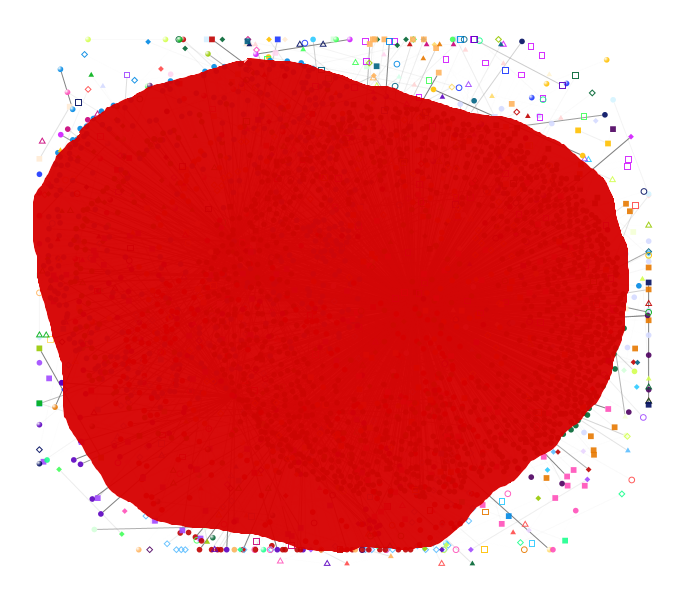
\includegraphics[width=0.9\textwidth]{img/floyd_social.png}
\end{figure}
\FloatBarrier

\FloatBarrier
\subsection{Работа алгоритма}
Как уже было отмечено ранее, работа алгоритма разбивается на три этапа, которые в дальнейшем будут рассмотрены по отдельности.

\begin{itemize}
  \item Анализ графа и выбор базовой вершины. 
  \item Обработка меньшего множества параллельным Беллманом-Фордом.
  \item Обработка большего множества методом динамического программирования
\end{itemize}

Первый и самый простой этап состоит в выборе базовой вершины. В качестве нее будет выбрана вершина с наибольшей степенью. После этого из этой вершины будет запущен обход в ширину, который найдет все вершины, отстоящие не более, чем на $K$ (в случае классической теории шести рукопожатий $K = 6$). Таким образом, все такие вершины попадают в большее множество $handleByBaseVertexSet$, которое будет обработано на третьем этапе алгоритма. Все остальные вершины попадают в меньшее множество $otherVertexSet$. Псевдокод этого этапа выглядит следующим образом

\FloatBarrier
\begin{algorithm}
\caption{Первая фаза алгоритма}\label{all_pairs_social1}
\begin{algorithmic}[1]
\Procedure{ConstructSets}{$G$}
\State {$baseVertex \gets $ Вершина максимальной степени}
\State {$dist \gets $ Запустить обход в ширину из $baseVertex$}
\State $handleByBaseVertexSet \gets \emptyset$
\algrenewcommand\algorithmicfor{\textbf{parfor}} 
\For{$i = 0$ to $|G.vertices| - 1$}
\algrenewcommand\algorithmicfor{\textbf{for}}
	\If {$dist[i] \leq K$ }
		\State $handleByBaseVertexSet.add(i)$
	\EndIf
\EndFor

\State $otherVertexSet \gets G.vertices \setminus handleByBaseVertexSet$
\State $otherVertexSet \gets otherVertexSet \cup  \left\{ {baseVertex}\right\}$
 
\State \textbf{return} $ baseVertex, handleByBaseVertexSet, otherVertexSet$
\EndProcedure

\end{algorithmic}
\end{algorithm}




В качестве алгоритма для обработки второго множества запустим параллельный обход в ширину (он же Беллман-Форд) для каждой из вершин этого множества. Иными словами, мы просто воспользуемся Алгоритмом 7 для множества вершин (для $otherVertexSet$). При этом исходя из наших эвристик мы предполагаем небольшие размеры множества, что позволяет думать об этом этапе как о значительно менее затратным по времени по сравнению с последним. Кроме того, значения расстояния, посчитанные обходом в ширину из базовой вершины нам помогут на третьем этапе, поэтому добавим в множество $otherVertexSet$ базовую вершину (чтобы в дальнейшем при обращений к глобальному массиву $dist$ в нем содержались корректные расстояния от базовой вершины).

Для поиска искомых значении для вершин множества $handleByBaseVertexSet$ воспользуемся методом динамического программирования. Но сперва обсудим основные принципы построения алгоритма и доказательство его корректности. 

Рассмотрим некоторую вершину, которая находится на расстояний $d$ от базовой вершины ($d \leq K$). То какие вершины для нее могут находится на расстоянии $i$? Это могут быть только те вершины, которые находятся на расстоянии $[i-d, \ i+d]$ от базовой. Иначе бы не выполнялось свойство, что путь кратчайший. С другой стороны, если рассмотреть некоторую вершины, расстояние до которой от базовой равняется $i$, то для всех вершин из множества $handleByBaseVertexSet$ верно, что кратчайшее расстояние от них до нее варьируется в промежутке $[i-K, \ i+K]$. 

 Предположим, что мы запустили обход в ширину из всех вершин большого множества. То какие вершины могут быть в слое с номером $i$? Ответ вытекает из рассуждений предыдущего абзаца - только вершины, расстояние от которых до базовой варьируется в промежутке $[i-K, \ i+K]$. То есть каждая из вершин будет принимать участие в не более, чем $2K+1$ слоях. То построим для каждого слоя обхода в ширину множество возможных вершин на этом слое. Это избавит нас от построения таких множеств в процессе работы алгоритма. И при этом общее количество вершин во всех слоях будет пропорционально числу вершин в графе (если учитывать, что $K$ - небольшое число, меньшее 7). 
 
 После того, как мы построили набор вершин для каждого из слоев мы можем воспользоваться структурой данных Frontier для эффективного распараллеливания процесса обработки ребер, исходящих из этих вершин. Однако к текущему моменту мы никак не воспользовались тем фактом, что вершины расположены близко друг к другу, и, может быть, существует эффективный технических прием для оптимальной обработки группы вершин. Такой подход существует и основан на идее динамического программирования и применения битовых векторов (bitset). Обратим внимание, что битовые вектора должны поддерживать битовые логические операции (конъюнкция, дизъюнкция и отрицание) и стандартные методы установки соответствующего бита и его получение.
 
 Будем поддерживать две следующие динамики. Значениями в полях массива будут битовые вектора --- это некоторая структура, где каждый из битов соответсвует вершине из множества $handleByBaseVertexSet$. 
 
 \begin{itemize}
  \item $mask[u][i]$ --- набор вершин, расстояние от которых до $u$ равно $i$ 
  \item $calc[u][i]$ --- набор вершин, расстояние от которых до $u$ меньше $i$
\end{itemize}
 
 Рассмотрим процесс пересчета значений динамики. Для подсчета текущего значения $mask[v][i]$ воспользуемся формулой (2.1). Суть формулы состоит в переборе всех ребер графа, входящих в текущую вершину и применение операции битовое "или" для соответствующих масок. При этом мы не должны учитывать данные для тех вершин, расстояние до которых уже посчитано (эта информация хранится в массиве $calc$).  
  
%mask[v][i] = \bigvee (mask[u][i - 1] where \exists edge u->v) AND (

\FloatBarrier
\begin{equation}
mask[v][i] = \neg calc[v][i - 1] \wedge \bigvee_{\exists (u, v) \in E} mask[u][i - 1] 
\end{equation}
\FloatBarrier

В свою очередь $calc$ пересчитывается согласно (2.2)
\FloatBarrier
\begin{equation}
calc[v][i] = calc[v][i - 1] \vee mask[v][i]
\end{equation}
\FloatBarrier

Псевдокод пересчета значений динамики представлен ниже. Обратим внимание, что для каждой вершины нам достаточно хранить всего $2K + 1$ битовых векторов. Однако для упрощения понимания псевдокода будем обращаться к $i$ слою вершины $u$ просто как $mask[u][i]$, при этом имея в виду эту значительную оптимизацию по памяти. Кроме того другим важным замечанием является то, что когда нам необходимо посчитать значения динамики для слоя $i$, то нам необходимо обрабатывать предыдущий слой. Таким образом в последнем цикле алгоритма для обработки $layerToCalc$ мы используем $frontierLayer \gets layerToCalc - 1$.

\FloatBarrier
\begin{algorithm}
\caption{Пересчет динамики}\label{all_pairs_social2}
\begin{algorithmic}[1]
\State $ K \gets 6$ \Comment{Максимальная глубина до базовой вершины}\ldots
\State

\Procedure{CalculateDistancesForBigSet}{$G, baseVertex, handleByBaseVertexSet$}
\State {$maxLayer \gets $ calculate max distance from baseVertex}
\State {$Frontiers \gets \left\{ {Frontier_0 \ldots Frontier_{maxLayer + K}}\right\} $} \Comment{Фронтир для каждого уровня обхода} 
\State {$VertexSets \gets \left\{ {VertexSet_0 \ldots VertexSet_{maxLayer + K}}\right\} $} \Comment{Набор вершин для каждого уровня} 
\State $mask\gets \left\{ {   \left\{ {bitVector(0) \ldots bitVector(0)}\right\}  \ldots \left\{ {bitVector(0) \ldots bitVector(0)}\right\} }\right\}$ 
\State $calc\gets \left\{ {   \left\{ {bitVector(0) \ldots bitVector(0)}\right\}  \ldots \left\{ {bitVector(0) \ldots bitVector(0)}\right\} }\right\}$
\State

\For{$i = 0$ to $maxLayer + K$}	
	\For{$j = dist[baseVertex][i] - K$ to $dist[baseVertex][i] + K$}		
		\State $Frontiers[j].pushEdgesOf(i)$
		\State $VertexSets[j].addVertex(i)$
	\EndFor
\EndFor
\State

\For{$v \in handleByBaseVertexSet $}
	\State $mask[v][0] \gets bitVector(bitNum(v))$ \Comment{Будем считать, что существует функция bitNum, которая по номеру вершины возвращает соответсвующий ей бит} 

\EndFor 
\State
\For{$layerToCalc = 1$ to $maxLayer + K$}
	\State $frontierLayer \gets layerToCalc - 1$ 
	\State {\Call {ProcessLayerLazy}{$G, Frontiers[frontierLayer], mask, layerToCalc$}}

	\algrenewcommand\algorithmicfor{\textbf{parfor}}
	\For{$v \in VertexSets[layerToCalc] $}
		\State {$calc[v][layerToCalc] \gets mask[v][layerToCalc] $}
		\If {$layerToCalc$ is not first layer for vertex $v$}
			\State $calc[v][layerToCalc - 1] \gets \lnot calc[v][layerToCalc - 1]$ 
			\State $mask[v][layerToCalc] \gets mask[v][layerToCalc] \land calc[v][layerToCalc - 1]$ 
			\State $calc[v][layerToCalc - 1] \gets \lnot calc[v][layerToCalc - 1]$ 
			\State $calc[v][layerToCalc] \gets calc[v][layerToCalc] \lor calc[v][layerToCalc - 1]$ 
		\EndIf

	\EndFor 
	\algrenewcommand\algorithmicfor{\textbf{for}}	
\EndFor 
\EndProcedure
\end{algorithmic}
\end{algorithm}
\FloatBarrier

Для полноты алгоритма осталось описать обработку текущего Frontier. Псевдокод этого этапа представлен ниже. В этом алгоритме мы снова (как и в алгоритмах из первой главы) пользуемся интерефейсом, который предоставляет библиотека для параллельных вычислений PASL. Напомню, что для взаимодействие между рабочими потоками существует служебные функции, дающие понять потокам необходимость разбиения фронтира для обработки на других ядрах или же понять обратное. 
\begin{algorithm}
\caption{Обработка Фронтира}\label{all_pairs_social3}
\begin{algorithmic}[1]

\Procedure{ProcessLayerLazy}{$G, Frontier, mask, layer, dists, baseVertex$}
\While {\algorithmicnot $Frontier.empty()$}
	\If {$hasIncomingQuery()$}
		\If {$Frontier.nbEdges() \leq cutoff$}
			\State $rejectQuery()$			
		\Else		
			\State $NewFrontier \gets \emptyset$
			\State $Frontier.split(NewFrontier)$
			\State \begin{varwidth}[t]{\linewidth}fork2(\par
        \hskip\algorithmicindent {\Call {ProcessLayerLazy}{$G, Frontier, mask, layer, dists, baseVertex$}},\par
        \hskip\algorithmicindent {\Call {ProcessLayerLazy}{$G, NewFrontier, mask, layer, dists, baseVertex$}});
      \end{varwidth}
		\EndIf
		
	\EndIf
	\State Frontier.iterNumber(pollingCutoff, updateFunction(mask, from, to, layer, dists, baseVertex))
\EndWhile
\EndProcedure
\State
\Procedure{UpdateFunction}{$mask, from, to, layer, dists, baseV$}
\If {HaveOnLayer(layer - 1, from, dists, baseV) \algorithmicand HaveOnLayer(layer, to, dists, baseV)} 
	
	\State $mask[to][layer] \gets mask[to][layer] \lor mask[from][layer - 1]$ \Comment Атомарно
\EndIf
\EndProcedure
\State
\Procedure{HaveOnLayer}{$layer, vertex, dists, baseV$}
\State \textbf{return} {$|layer - dists[baseV][vertex]| \leq K$}  
\EndProcedure

\end{algorithmic}
\end{algorithm}


\FloatBarrier
Наконец, как по имеющимся данным динамики восстановить ответ? Для каждого значения $mask[u][i]$ найдем единичные биты в маске. Установленный в единицу бит $j$ говорит о том, что расстояние от вершины из "большого" множества с идентификатором $j$ до вершины $u$ равно $i$. Таким образом, мы сможем полностью восстановить ответ для каждой вершины. 

Важным замечанием к коду является последовательность выполнения циклов в последней части алгоритма. Рассмотрим на примере как происходит обращение к памяти в двух различных вариантах (Алгоритм \ref{fill_way_1} и Алгоритм \ref{fill_way_2}), при этом выполняющих совершенно одно и то же. Заметим, что в этих алгоритмах отличается порядок параллельных циклов. 

\FloatBarrier
\begin{algorithm}
\caption{Заполнение массива ответа по динамика (1 вариант)}\label{fill_way_1}
\begin{algorithmic}[1]

\Procedure{FillDistances1}{$G, dist, mask, baseVertex, handleByBaseVertexSet$}
\algrenewcommand\algorithmicfor{\textbf{parfor}}
\For{$v = 0$ to $|G.vertices|$}
\algrenewcommand\algorithmicfor{\textbf{for}}
	\For{$j = dist[baseVertex][i] - K$ to $dist[baseVertex][i] + K$}	
		\algrenewcommand\algorithmicfor{\textbf{parfor}}	
		\For{$u \in handleByBaseVertexSet$}
			\If {$mask[v][j].getBit(bitNum(u)) = 1$}
				\State $dist[u][v] = j$		
			\EndIf	
		\EndFor
		\algrenewcommand\algorithmicfor{\textbf{for}}
	\EndFor
\EndFor 
\EndProcedure
\end{algorithmic}
\end{algorithm}

\FloatBarrier
\begin{algorithm}
\caption{Заполнение массива ответа по динамика (2 вариант)}\label{fill_way_2}
\begin{algorithmic}[1]

\Procedure{FillDistances2}{$G, dist, mask, baseVertex, handleByBaseVertexSet$}
\algrenewcommand\algorithmicfor{\textbf{parfor}}
\For{$u \in handleByBaseVertexSet$}
\algrenewcommand\algorithmicfor{\textbf{for}}
	\For{$j = dist[baseVertex][i] - K$ to $dist[baseVertex][i] + K$}	
		\algrenewcommand\algorithmicfor{\textbf{parfor}}	
		\For{$v = 0$ to $|G.vertices|$}
			\If {$mask[v][j].getBit(bitNum(u)) = 1$}
				\State $dist[u][v] = j$		
			\EndIf	
		\EndFor
		\algrenewcommand\algorithmicfor{\textbf{for}}
	\EndFor
\EndFor 
\EndProcedure
\end{algorithmic}
\end{algorithm}
\FloatBarrier

Так как некоторый $mask[i][j]$ представляет из себя область последовательной памяти, то в случае первого варианта процессор будет работать при вызове методов $getBit$ именно с последовательной памятью, в то время как вторая версия будет обращаться к различным элементам матрицы $mask$ и тем самым к разным участками памяти, что, заметно медленнее в силу специфик устройства вычислительной машины. Это замечание было подтверждено и на практике - алгоритм со второй реализаций работает (на той же машине, которая упоминалась в контексте тестирования параллельного Беллмана-Форда) в среднем в 1.5 раза дольше, чем с первым вариантом.

Итого, псевдокод алгоритма выглядит следующим образом.

\FloatBarrier
\begin{algorithm}
\caption{Параллельная версия для социальных графов}\label{all_pairs_social}
\begin{algorithmic}[1]

\Procedure{AllPairsSocialPar}{$G$}
\State $dist\gets \left\{ {   \left\{ {\infty \ldots \infty}\right\}  \ldots \left\{ {\infty \ldots \infty}\right\} }\right\}$
\State {$ baseVertex, handleByBaseVertexSet, otherVertexSet \gets ConstructSets(G)$}
\State {\Call {AllPairsPar1}{$G, otherVertexSet, dist$}} \Comment {Наивный алгоритм для множества вершин}
\State {\Call {CalculateDistancesForBigSet}{$G, baseVertex, otherVertexSet, dist$}}
\State {\Call {FillDistances1}{$G, dist, mask, baseVertex, handleByBaseVertexSet$}}
\State \textbf{return} $dist$ 
\EndProcedure

\end{algorithmic}
\end{algorithm}


\FloatBarrier
\subsection{Сравнение с наивными версиями}

Обратим внимание, что асимптотически этот подход не отличается от предыдущих. Однако у него есть ряд преимуществ. 

\begin{itemize}
  \item Пересчет расстояний для группы вершин выполняется быстрее за счет битовых операций. Хоть это и не сказывается на асимптотику, но на практике дает заметный выигрыш. 
  \item Все битовые операции выполняются без выделения дополнительной памяти. При этом изменяются уже созданные поля в массиве для подсчета динамики
  \item Так как каждый из фронтиров уже построен, то нам не приходится строить следующий фронтир по предыдущему в процессе обработки
  \item Каждый из получившихся фронтиров довольно большой, что увеличивает его способность к параллелизации
  \item Все остальные этапы также хорошо параллелятся
\end{itemize}

Таким образом мы имеем полные основания предполагать, что этот алгоритм на практике покажет заметно лучшие результаты по сравнению с предыдущими версиями. 

Для подтверждения этих гипотез все алгоритмы были реализованы и протестированы на той же машине, о которой шла речь в предыдущей главе в контексте Беллмана-Форда.

В качестве графов для тестирования были взяты подграф твиттера из 81306 вершинами и 4841532 ребрами и граф научной социальной сети Slashdot из 82168 вершин и 877286 ребер. При этом каждое из ребер графов считалось неориентированным. Для сравнения были взяты два алгоритма --- стандартная параллельная версия и последний описанный алгоритм. Результаты запуска приведены в таблице \ref{table:algo_floyd_comparison}.   


\FloatBarrier
\begin{table}[H]
\centering

\begin{tabular}{l|c|c}  
Алгоритм & Twitter & Slashdot\\
\hline\hline
Стандартная параллельная версия & 427.217 & 254.567 \\  
Алгоритм для социальных графов & 191.232 & 169.393  \\
\hline
\end{tabular}

\caption{Сравнение алгоритмов}
\label {table:algo_floyd_comparison}
\end{table}
\FloatBarrier

Как мы видим мы получили значительный прирост производительности в обоих случаях, что подтверждает наши ожидания относительно эффективности последнего подхода.

\FloatBarrier
\subsection{Модификации}

Данный алгоритм специализирован для неориентированных невзвешенных графов социальных сетей. Однако существует небольшая модификация алгоритма, которая позволяет без значительных изменений применять алгоритм для взвешенных графов графов социальных сетей, в которых веса ребер ограничены небольшой константой $c$. 

Идея заключается в представлении каждого ребра с весом $d$ в виде цепочки из $d$ ребер. Пример такого преобразования представлен на рисунке \ref{edge_modification}. После такого преобразования граф может быть обработан нашим алгоритмом.

\FloatBarrier

\begin{figure}[h]
\caption{Пример преобразования ребра}
\label{edge_modification}
\centering
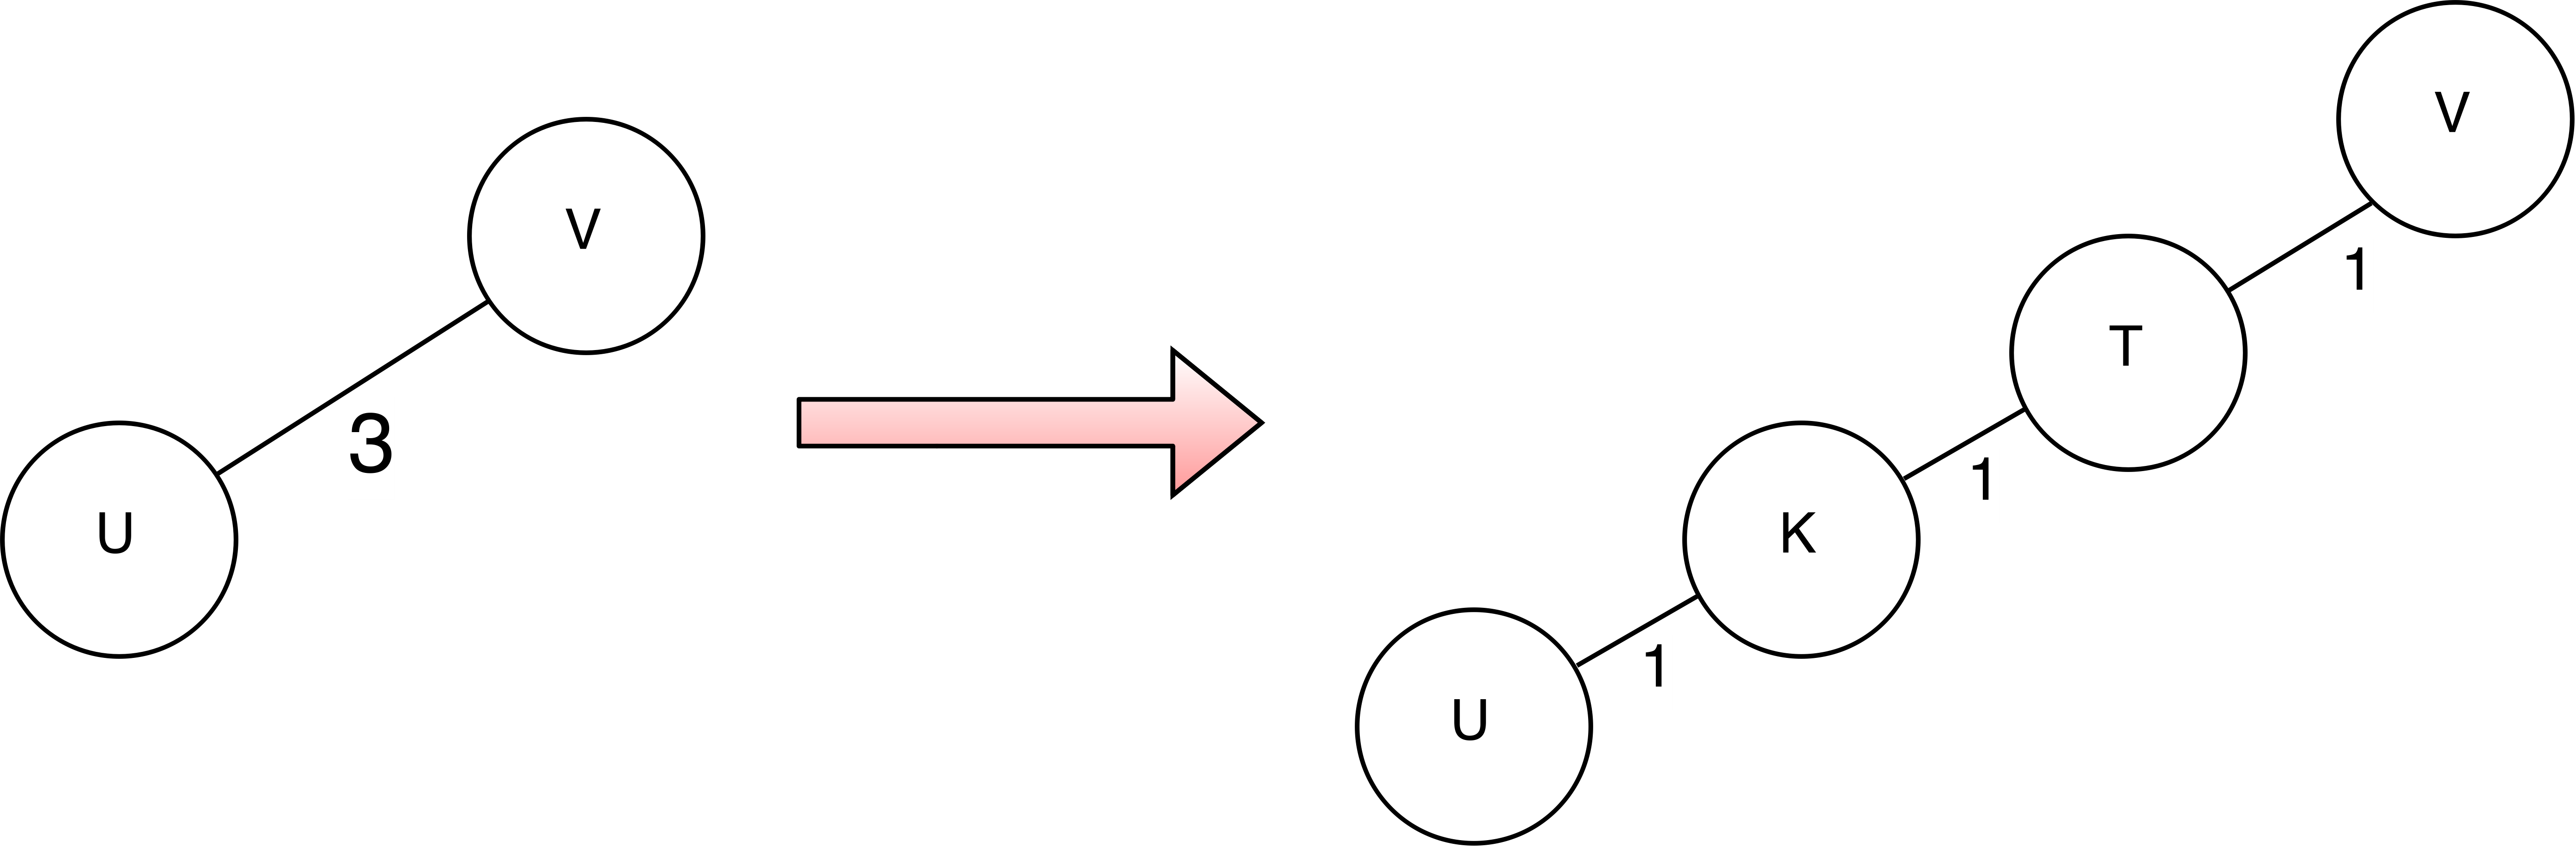
\includegraphics[width=0.9\textwidth]{img/floyd_social_modification.png}
\end{figure}
\FloatBarrier

В этой модификации алгоритм в худшем случае будет работать за $O(c \ VE)$ за счет увеличения числа ребер в $c$ раз.

\FloatBarrier
\section{Выводы}
Таким образом в этой части мы описали алгоритм для поиска кратчайшего расстояния на разреженных графах в общем случае (наивная версия) и для частного случая для социальных графов. При этом последний показал свою высокую эффективность на практике на реальных графах социальных сетей.
\FloatBarrier
